%%%%%%%%%%%%%%%%%%%%%%%%%%%%%%%%%%%%%%%%%
% FRI Data Science_report LaTeX Template
% Version 1.0 (28/1/2020)
% 
% Jure Demšar (jure.demsar@fri.uni-lj.si)
%
% Based on MicromouseSymp article template by:
% Mathias Legrand (legrand.mathias@gmail.com) 
% With extensive modifications by:
% Antonio Valente (antonio.luis.valente@gmail.com)
%
% License:
% CC BY-NC-SA 3.0 (http://creativecommons.org/licenses/by-nc-sa/3.0/)
%
%%%%%%%%%%%%%%%%%%%%%%%%%%%%%%%%%%%%%%%%%


%----------------------------------------------------------------------------------------
%	PACKAGES AND OTHER DOCUMENT CONFIGURATIONS
%----------------------------------------------------------------------------------------
\documentclass[fleqn,moreauthors,10pt]{ds_report}
\usepackage[english]{babel}

\graphicspath{{fig/}}




%----------------------------------------------------------------------------------------
%	ARTICLE INFORMATION
%----------------------------------------------------------------------------------------

% Header
\JournalInfo{Machine Learning for Data Science, 2025}

% Interim or final report
%\Archive{Interim report}
%\Archive{Final report} 

% Article title
\PaperTitle{
Implementation and Evaluation of Classification Trees and Random Forests for Binary Classification
}

% Authors (student competitors) and their info
\Authors{Teodora Taleska}

% Advisors
%\affiliation{\textit{Advisors: prof. Janez Novak, dr. Alica Kavčič}}

% Keywords
%\Keywords{Classification Trees, Random Forests, Binary Classification, Gini Impurity, Variable Importance, Bootstrap Sampling}
%\newcommand{\keywordname}{Keywords}


%----------------------------------------------------------------------------------------
%	ABSTRACT
%----------------------------------------------------------------------------------------

\Abstract{
This report presents the implementation and evaluation of classification trees and random forests for binary classification tasks, specifically applied to the TKI resistance FTIR spectral data set. The methods utilized include building classification trees using Gini impurity for splitting and random forests with bootstrap sampling and random variable selection. The performance of the models was assessed using misclassification rates and standard errors, and variable importance was analyzed using permutation-based methods. The feature importance approach was extended by assessing combinations of three variables and tree structure-based importance. The findings offer insights into the effectiveness of these models and their performance in predictive tasks.
}

%----------------------------------------------------------------------------------------

\begin{document}

% Makes all text pages the same height
\flushbottom 

% Print the title and abstract box
\maketitle 

% Removes page numbering from the first page
\thispagestyle{empty} 

%----------------------------------------------------------------------------------------
%	ARTICLE CONTENTS
%----------------------------------------------------------------------------------------

\section*{Introduction}

The objective of this project is to implement classification trees and random forests from scratch and evaluate their performance on the TKI resistance FTIR spectral dataset. The dataset consists of spectral measurements across multiple wavelengths for different cell lines, with a binary classification target.

The project is divided into three parts:

\begin{enumerate}
\item Building and evaluating classification trees and random forests – Implementing the models, computing misclassification rates, and quantifying uncertainty.
\item Variable importance analysis – Implementing permutation-based feature importance to identify the most relevant spectral variables.
\item Extending feature importance analysis – Assessing variable interactions and analyzing tree structures to derive the most significant combinations of three variables.
\end{enumerate}

This report details the implementation methodology, experimental results, and conclusions drawn from evaluating classification trees and random forests on the dataset.

%------------------------------------------------

\section*{Part 1: Misclassification Rates and Uncertainty}

\subsection*{Methodology}

\subsubsection*{Classification Trees}

In this project, \textbf{classification trees} were implemented, where the splits were made to minimize the \textbf{Gini impurity}. The Gini impurity measures the likelihood of an incorrect classification of a randomly chosen element if it was randomly labeled according to the class distribution in the subset\cite{MLPP}. The formula for Gini impurity is:

\[
\text{Gini}(D) = 1 - \sum_{c=1}^{C} \hat{\pi}_c^2
\]
where:
\begin{itemize}
    \item \( D \) is the dataset at a node,
    \item \( C \) is the number of classes,
    \item \( \hat{\pi}_c \) is the proportion of data points in \( D \) that belong to class \( c \).
\end{itemize}

The goal of the tree is to recursively partition the data into subsets that are as pure as possible (i.e., containing mostly one class), thereby reducing the Gini impurity at each split.

%Additionally, the \textbf{misclassification rate} was used as an error measure to evaluate the quality of the splits. The misclassification rate is defined as\cite{MLPP}:
%
%\[
%\text{Misclassification Rate} = 1 - \hat{\pi}_{\hat{y}}
%\]
%
%where:
%\begin{itemize}
%    \item \( \hat{y} = \arg\max_c \hat{\pi}_c \) is the most probable class label in the subset,
%    \item \( \hat{\pi}_{\hat{y}} \) is the proportion of data points in \( D \) that belong to the most probable class.
%\end{itemize}

\subsubsection*{Random Forests}


Random forests are an ensemble learning method designed to reduce the variance of predictions by averaging the outputs of multiple decision trees. Each tree is trained on a different subset of the data, chosen randomly with replacement (a technique known as \textbf{bagging})\cite{MLPP}. The final prediction is computed as:

\[
f(x) = \frac{1}{M} \sum_{m=1}^{M} f_m(x),
\]

where \( f_m(x) \) is the prediction of the \( m \)-th tree, and \( M \) is the total number of trees in the forest.

To further reduce correlation between trees, random forests introduce randomness in two ways:
\begin{itemize}
    \item \textbf{Random subsets of data}: Each tree is trained on a bootstrap sample of the dataset.
    \item \textbf{Random subsets of features}: At each split, only a random subset of features is considered.
\end{itemize}

This decorrelation improves the model's predictive accuracy and robustness.


\subsubsection*{Quantifying Uncertainty}


To quantify the uncertainty of the estimates, we compute both the \textbf{misclassification rate (MR)} and the \textbf{standard error}. The misclassification rate measures the proportion of incorrectly classified samples\cite{MLPP}, while the standard error provides an estimate of the uncertainty associated with this rate.

The misclassification rate is calculated as:

\[
\text{MR} = 1 - \frac{1}{N} \sum_{i=1}^{N} \mathbb{I}(y_i = \hat{y}_i),
\]
where:
\begin{itemize}
    \item \( y_i \) is the true label for the \( i \)-th sample,
    \item \( \hat{y}_i \) is the predicted label for the \( i \)-th sample,
    \item \( N \) is the total number of samples,
    \item \( \mathbb{I}(\cdot) \) is the indicator function, which equals 1 if the condition is true and 0 otherwise.
\end{itemize}

The standard error of the misclassification rate is calculated as:

\[
\text{Standard Error} = \frac{\sigma}{\sqrt{N}},
\]
where:
\begin{itemize}
    \item \( \sigma \) is the standard deviation of the misclassification errors (\( y_i \neq \hat{y}_i \)),
    \item \( N \) is the total number of samples.
\end{itemize}


The misclassification rate provides a point estimate of the model's error, while the standard error measures the uncertainty of this estimate. Together, they allow us to assess not only how well the model performs but also how reliable the performance estimate is. For example, a low misclassification rate with a small standard error indicates both high accuracy and high confidence in the estimate. Conversely, a low misclassification rate with a large standard error suggests that the estimate may not be reliable due to high variability.


\subsection*{Results}

\subsubsection*{Decision Tree Misclassification Rates}

The decision tree model achieved a \textbf{training misclassification rate of \(0.0 \pm 0.0\)}, indicating perfect performance on the training data. However, on the test set, the misclassification rate increased to \(\mathbf{0.367 \pm 0.062}\). This suggests that the decision tree is overfitting the training data, as it performs well on the training set but poorly on the test set. The relatively high standard error on the test set indicates some variability in the model's performance.


\subsubsection*{Random Forest Misclassification Rates}

The random forest model, built with \textbf{100 trees}, achieved a \textbf{training misclassification rate of \(0.0 \pm 0.0\)}, similar to the decision tree. However, on the test set, the random forest performed significantly better, with a misclassification rate of \(\mathbf{0.217 \pm 0.053}\). This demonstrates that the random forest generalizes better to unseen data compared to the decision tree, reducing overfitting and improving test performance. The lower standard error also indicates more consistent performance across different test samples.

\subsubsection*{Misclassification vs. Number of Trees}


The plot below shows how the misclassification rate on the test set changes as the number of trees in the random forest increases. The shaded region represents the \textbf{standard error} of the misclassification rate, providing a measure of uncertainty.
\begin{figure}[h!]
    \centering
    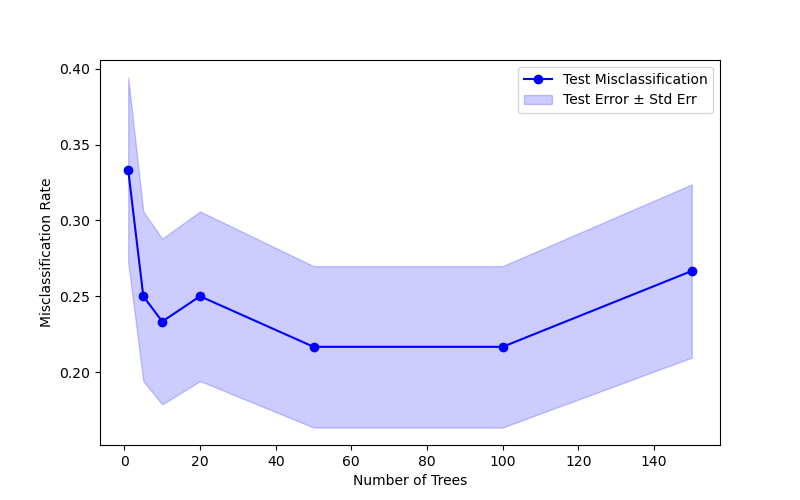
\includegraphics[width=0.5\textwidth]{fig/misclassification_vs_trees}
    \caption{Misclassification Rate vs. Number of Trees in Random Forest}
    \label{fig:misclassification_plot}
\end{figure}
From Figure~\ref{fig:misclassification_plot}, we observe the following:
\begin{itemize}
    \item As the number of trees increases, the misclassification rate on the test set initially decreases, reaching a minimum at around \textbf{50 trees}.
    \item Beyond 50 trees, the misclassification rate stabilizes, with no significant improvement in performance.
    \item The standard error remains relatively constant, indicating that the model's performance is consistent across different numbers of trees once the forest is sufficiently large.
\end{itemize}

This behavior aligns with the theory of random forests: increasing the number of trees reduces variance and improves generalization, but beyond a certain point, the gains diminish. The results suggest that \textbf{50 trees} are sufficient for this dataset, as adding more trees does not significantly improve performance.

%------------------------------------------------

\section*{Part 2: Variable Importance Analysis}

\subsection*{Methodology}

\subsubsection*{Permutation-Based Feature Importance}

Variable importance in random forests can be computed using out-of-bag (OOB) samples. For each tree in the forest, the OOB samples (data not used to train the tree) are passed through the tree, and the prediction accuracy is recorded. To measure the importance of a variable, its values in the OOB samples are randomly permuted, and the accuracy is recomputed. The decrease in accuracy due to this permutation is averaged over all trees and used as the importance measure for the variable. This method effectively simulates the removal of the variable's contribution, providing a robust estimate of its predictive strength\cite{ESL}.

\subsection*{Results}


\subsubsection*{Variable Importance and Root Frequency}

To analyze the importance of features in the dataset, we computed the variable importance for a random forest with \( n = 100 \) trees. For comparison, we also calculated the frequency of features appearing as the root split in 100 non-random trees trained on randomized data. The results are visualized in the Figure~\ref{fig:variable_importance}.

\begin{figure}[h!]
    \centering
    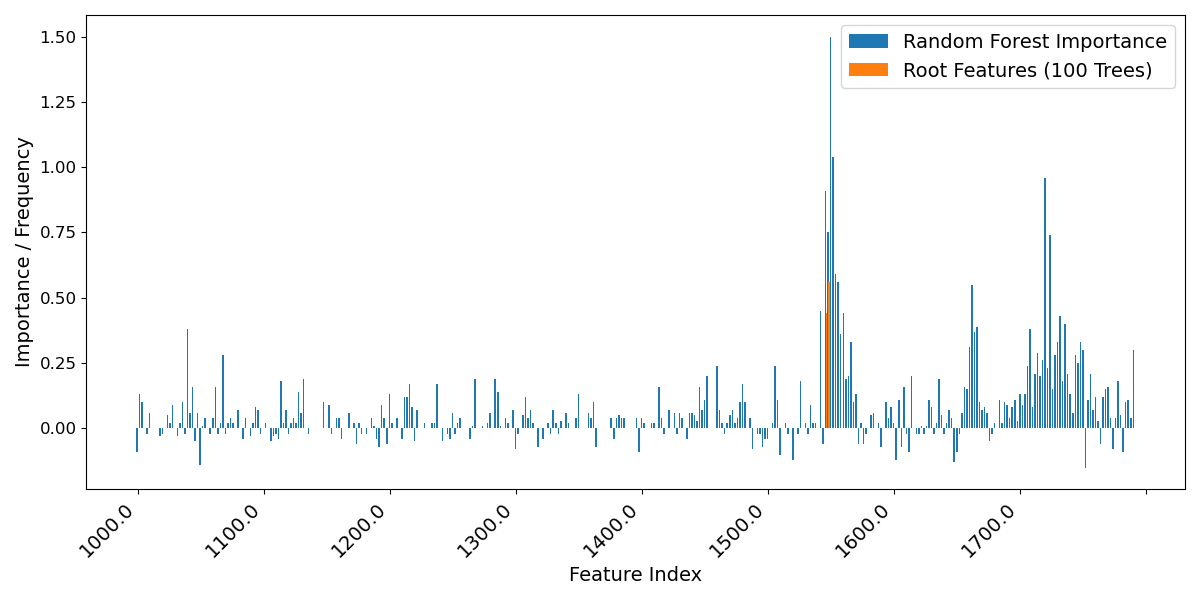
\includegraphics[width=0.5\textwidth]{fig/variable_importance}
    \caption{Variable Importance (Random Forest) vs. Root Frequency (Non-Random Trees)}
    \label{fig:variable_importance}
\end{figure}
The plot shows the following key observations:
\begin{itemize}
    \item Only two features appeared as the root split in the non-random trees:
        \begin{itemize}
            \item \textbf{Feature 1548.0}: Ranked as the \textbf{5th most important} by the random forest, this feature appeared as the root split in \textbf{56\%} of the non-random trees.
            \item \textbf{Feature 1546.0}: Ranked as the \textbf{4th most important} by the random forest, this feature appeared as the root split in \textbf{44\%} of the non-random trees.
        \end{itemize}
    \item The random forest identified additional important features (e.g., 1550.0, 1552.0, 1720.0) that did not appear as root splits in the non-random trees, highlighting the ability of random forests to capture complex interactions beyond simple root splits.
\end{itemize}


%------------------------------------------------

\section*{Part 3: Extended Variable Importance}


\subsubsection*{Extended Variable Importance to Combinations of Three Variables}
To extend variable importance to combinations of three variables, we implemented the \textbf{importance3()} method. This method evaluates the importance of feature combinations by permuting the values of three features simultaneously and measuring the resulting drop in prediction accuracy. Specifically:
\begin{itemize}
    \item For each combination of three features, the values of these features are shuffled in the out-of-bag (OOB) samples.
    \item The decrease in accuracy due to this permutation is averaged over all trees in the forest, providing a measure of the importance of the combination.
\end{itemize}
This approach captures interactions between features, which are often critical in complex datasets like the TKI resistance data. We applied this method to a random forest with \( n = 1000 \) trees and compared its performance to the original single-feature importance method.

\subsubsection*{Tree Structure-Based Importance}
In scenarios where the original data is unavailable but a pre-built forest exists, we implemented the \textbf{importance3\_structure()} method. This method identifies the best combination of three variables by analyzing the structure of the trees in the forest:
\begin{itemize}
    \item For each tree, we extract the features used in its splits and count how often each combination of three features appears together.
    \item The combination with the highest frequency across all trees is selected as the most important.
\end{itemize}

\subsection*{Results}

\subsubsection*{Comparison of Classification Trees}
We trained classification trees using the top 3 features identified by three different methods:
\begin{itemize}
    \item \textbf{Single-Feature Importance}: The top 3 features were \textbf{['1548.0', '1552.0', '1550.0']}, achieving an accuracy of \textbf{58.33\%}.
    \item \textbf{3-Feature Combination Importance}: The top combination was \textbf{['1660.0', '1550.0', '1558.0']}, achieving an accuracy of \textbf{63.33\%}.
    \item \textbf{Tree Structure-Based Importance}: The top combination was \textbf{['1784.0', '1546.0', '1554.0']}, achieving an accuracy of \textbf{63.33\%}.
\end{itemize}

\subsubsection*{Key Observations}
\begin{itemize}
    \item The classification trees built using the top 3-feature combinations (\textbf{importance3} and \textbf{importance3\_structure}) outperformed the tree built using the top 3 single features, achieving an accuracy of \textbf{63.33\%} compared to \textbf{58.33\%}.
    \item Both 3-feature combination methods (\textbf{importance3} and \textbf{importance3\_structure}) performed equally well, suggesting that considering feature interactions is crucial for improving model performance.
    \item The \textbf{importance3\_structure} method, which relies on the structure of the pre-built forest, identified a different combination of features (\textbf{['1784.0', '1546.0', '1554.0']}) but achieved the same accuracy as \textbf{importance3}. This demonstrates that the tree structure-based approach is effective even without access to the original data.
\end{itemize}

\subsubsection*{Why the Tree Structure-Based Method Works Well}

Since we only have access to the random forest and not the original data, the method analyzes all splits in the trees to extract the features used. By tracking the frequency of 3-feature combinations across the forest, it selects the combination that appears most frequently. This works well because features that are frequently used together in splits are likely to capture important patterns in the data and effectively partition it. In a random forest, features that are frequently used in splits are those that provide the most information gain or Gini impurity reduction. If a combination of features is frequently used together, it suggests that these features collectively contribute to better splits, meaning they capture important patterns in the data.


\subsubsection*{Why Counting Frequencies at All Levels is Important}

Counting frequencies of all features at every level, rather than just high-level features, ensures a comprehensive understanding of the data. High-level splits capture global patterns, while lower-level splits refine these with localized, nuanced interactions. Ignoring lower levels risks missing critical feature combinations that only become apparent deeper in the trees. Additionally, random forests introduce variability across trees, so evaluating all levels ensures robustness and avoids bias. This approach balances global and local importance, capturing hierarchical interactions and leading to more accurate feature selection and data partitioning.







%------------------------------------------------

%\section*{Discussion}


%------------------------------------------------


%----------------------------------------------------------------------------------------
%	REFERENCE LIST
%----------------------------------------------------------------------------------------
\bibliographystyle{unsrt}
\bibliography{report}


\end{document}